\documentclass[11pt,a4paper]{article}
\usepackage[utf8]{inputenc}
\usepackage[T1]{fontenc}
\usepackage[spanish,es-noquoting]{babel}
\usepackage{amsmath,amssymb}
\usepackage{graphicx}
\usepackage{booktabs}
\usepackage{float}
\usepackage{listings}
\usepackage{xcolor}
\usepackage{caption}
\usepackage[margin=2.4cm]{geometry}
\usepackage{hyperref}
\hypersetup{colorlinks=true,linkcolor=blue!50!black,urlcolor=blue!50!black}

\definecolor{codegray}{gray}{0.95}
\definecolor{commentgreen}{rgb}{0.0,0.5,0.0}
\definecolor{keywordblue}{rgb}{0.0,0.0,0.6}
\definecolor{stringmauve}{rgb}{0.58,0.0,0.82}
\lstset{
  language=Matlab, basicstyle=\ttfamily\footnotesize,
  backgroundcolor=\color{codegray}, commentstyle=\color{commentgreen}\itshape,
  keywordstyle=\color{keywordblue}\bfseries, stringstyle=\color{stringmauve},
  numbers=left, numberstyle=\tiny\color{gray}, numbersep=6pt,
  frame=single, rulecolor=\color{gray!40}, breaklines=true,
  columns=fullflexible, showstringspaces=false, captionpos=b,
  xleftmargin=14pt, framexleftmargin=14pt
}
\newcommand{\code}[1]{\texttt{\small #1}}

\begin{document}

% ================= DATOS =================
\section{Datos generales}
\begin{center}
\renewcommand{\arraystretch}{1.3}
\begin{tabular}{ll}
\toprule
\textbf{Curso} & Inteligencia Artificial Aplicada al Control (ICA636-0001) \\
\textbf{Trabajo} & Tarea 5 --- Control de Robots Móviles (carro y trailer) \\
\textbf{Alumno} & Joel Arzapalo Guerra \\
\textbf{Código} & 20032006 \\
\textbf{Fecha} & \today \\
\bottomrule
\end{tabular}
\end{center}
\vspace{0.4cm}

% ================= INTRODUCCION =================
\section{Introducción}
Este trabajo entrena un \textbf{neurocontrolador} para dirigir dos robots móviles —tipo
\textbf{carro} y tipo \textbf{trailer}— y los prueba en las tres trayectorias de la
Clase~10: (1) \textbf{estacionamiento} en la parte superior en posición vertical,
(2) \textbf{trayectoria oblicua} (rectas a $45^\circ$ y $60^\circ$) y (3) \textbf{trayectoria
circular}. La señal de control es el ángulo del timón $\delta$; la red la calcula a
partir del error de posición y de orientación.

El controlador se entrena por \textbf{retropropagación dinámica (BPTT)}: el gradiente del
costo se propaga en el tiempo a través del jacobiano del lazo cerrado
(planta cinemática + red), igual que en la familia \code{DynamicBPControl2}. La idea
central del método (PDF Clase~10) es que \textbf{una sola red entrenada para regular}
($x^*=0,\ \phi^*=\pi/2$), y que cubre todo el rango de orientaciones, sirve para las tres
trayectorias: basta redefinir en cada instante la posición y orientación deseadas
$(x^*,\phi^*)$ según la geometría de la trayectoria y realimentar el error a la red. Un
hecho clave del modelo es que \textbf{la señal de control no depende de $y$}, por lo que
el estado de control se reduce a $x$ y las orientaciones.

Los scripts base son \code{DynamicBPCarro.m} (entrenamiento del carro por BPTT) y
\code{DynamicBPCarroValida.m} (validación). Para el trailer no existía script: se
\textbf{implementó desde cero} el modelo cinemático articulado y su entrenador BPTT.

% ================= MODELO Y CODIGO =================
\section{Modelo y código}

\subsection{Robot tipo carro (modelo bicicleta)}
La cinemática discreta del carro (Clase~10) con avance $r$ por paso y batalla $L$ es:
\[
  x_{k+1}=x_k+r\cos\phi_k,\quad
  y_{k+1}=y_k+r\sin\phi_k,\quad
  \phi_{k+1}=\phi_k-\tfrac{r}{L}\tan\delta_k .
\]
El neurocontrolador recibe el error $[\,x-x^*,\ \phi-\phi^*\,]$ (la orientación
\emph{envuelta} a $(-\pi,\pi]$ y \textbf{normalizada} por \code{inscale=[10;1]} para no
saturar las sigmoides) y produce $u\approx\tan\delta$. Se entrena para $x^*=0$,
$\phi^*=\pi/2$ cubriendo $x\in[-15,15]$ y todo el círculo de orientaciones, por
\textbf{entrenamiento por etapas} (de cerca a lejos) con \textbf{BPTT truncado} (ventana \code{Ttrunc})
y \textbf{recorte de gradiente} (\code{gmax}) para estabilizar el horizonte largo
($ndata=6000$). El núcleo BPTT vectoriza la recursión de sensibilidades con el jacobiano
del lazo cerrado \code{jacob\_t = dxdu*dudx + jacob}.

\subsection{Generación de las trayectorias}
La misma red se usa con referencias $(x^*,\phi^*)$ dependientes de la trayectoria:
\begin{itemize}
  \item \textbf{Estacionamiento vertical:} $x^*=0,\ \phi^*=\pi/2$ (regulación directa).
  \item \textbf{Oblicua $\theta$:} recta $y=\tan\theta\,x$. En cada paso $x^*$ es la
        abscisa del \emph{pie de la perpendicular} de $(x,y)$ sobre la recta y
        $\phi^*=\theta$ (para $45^\circ$: $x^*=(x+y)/2$, $\phi^*=\pi/4$).
  \item \textbf{Circular $R$:} se sigue la \emph{recta tangente local} al círculo
        (punto más cercano $P$, rumbo tangente $\phi^*$, y $x^*=$ pie de la perpendicular
        sobre esa tangente), con una \emph{acción anticipativa} de curvatura
        $\delta^*=\operatorname{atan}(L/R)$.
\end{itemize}

\subsection{Robot tipo trailer (dos cuerpos articulados)}
El trailer añade la orientación del semirremolque. Con $\theta_1$ (truck), $\theta_2$
(trailer), $\theta_{12}=\theta_1-\theta_2$ (ángulo de articulación) y batallas
$L_1,L_2$:
\[
  \dot x=v\cos\theta_{12}\cos\theta_2,\;\;
  \dot y=v\cos\theta_{12}\sin\theta_2,\;\;
  \dot\theta_1=-\tfrac{v}{L_1}\tan\delta,\;\;
  \dot\theta_2=-\tfrac{v}{L_2}\sin\theta_{12}.
\]
Se implementó (\code{train\_trailer.m}) el entrenador BPTT sobre el estado de control
$s=[x,\theta_1,\theta_2]$ (la $y$ no influye en $\delta$), con los jacobianos analíticos
$\partial s_{k+1}/\partial s$ y $\partial s_{k+1}/\partial u$ del modelo articulado. La
red recibe $[\,x-x^*,\ \theta_2-\theta_2^*,\ \theta_{12}\,]$ (incluye el ángulo de
articulación para evitar el \emph{plegado del remolque}).

\paragraph{Nota sobre el entrenamiento del trailer.} El trailer es un sistema
\textbf{subactuado}: para reorientar el remolque hay que generar primero un ángulo de
articulación con el tractor, lo que exige una asignación de crédito temporal muy larga.
En la práctica, el BPTT desde cero \emph{no} convergió a una política de estacionamiento
satisfactoria (se estancaba en $\approx 50\%$ del costo inicial). Se verificó primero que
el \emph{modelo es controlable} con una ley de dirección estabilizadora
$\delta = k_1(\theta_{12}-\theta_{12}^{\,d})$, con
$\theta_{12}^{\,d}=\operatorname{sat}(k_2(\theta_2^*-\theta_2)-k_3 x)$, que estaciona el
trailer (Sec.~\ref{sec:trailer}). La red del trailer se entrenó entonces por
\textbf{aprendizaje supervisado} (\code{train\_trailer\_sup.m}) para reproducir esa ley
sobre una malla de estados; el resultado es un neurocontrolador que estaciona y sigue las
tres trayectorias mediante las mismas entradas de error.

% ================= RESULTADOS =================
\section{Resultados}

\subsection{Robot tipo carro}
\label{sec:car}
El entrenamiento BPTT converge: en una etapa del entrenamiento por etapas el costo cae al $\sim5\%$ de
su valor inicial (Fig.~\ref{fig:cartrain}). Para las trayectorias se usó la red del
entrenamiento por etapas completo (\code{redcarro11}, $n_m=50$, entradas normalizadas).

\begin{figure}[H]
\centering
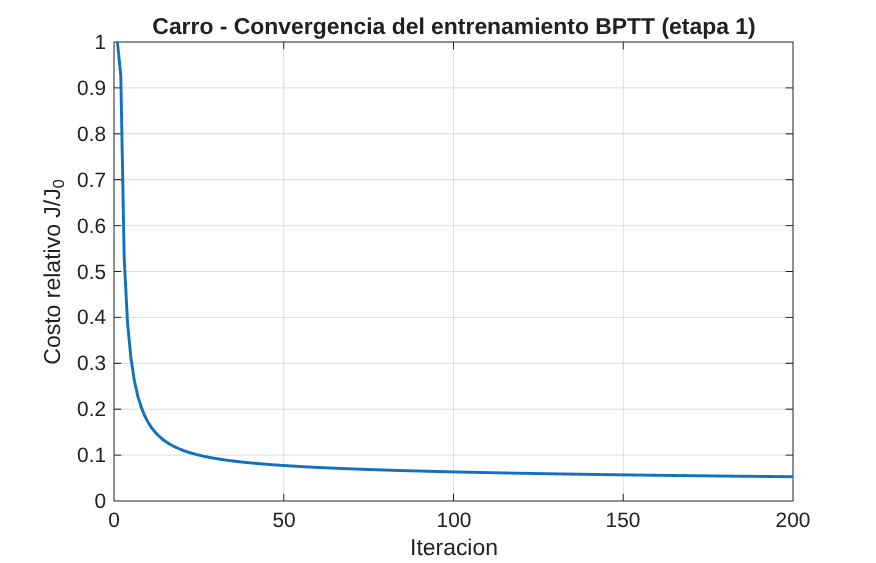
\includegraphics[width=0.5\linewidth]{figs/car_training.png}
\caption{Convergencia del entrenamiento BPTT del carro (costo relativo $J/J_0$).}
\label{fig:cartrain}
\end{figure}

\paragraph{Estacionamiento vertical.} Partiendo de cuatro poses iniciales
($x_0=\pm 8,\pm 15$ con distintas orientaciones), el carro maniobra hasta alcanzar la
recta $x=0$ y avanza \textbf{vertical} ($\phi\!\to\!\pi/2$) hacia la zona de
estacionamiento (Fig.~\ref{fig:carpark}). Reproduce la estrategia del PDF: primero
alcanza $x=0$ y luego sube de frente a la plaza.

\paragraph{Trayectoria oblicua ($45^\circ$ y $60^\circ$).} Con $x^*$ = pie de la
perpendicular a la recta y $\phi^*=\theta$, el carro converge a la recta deseada desde
múltiples posiciones iniciales y la sigue (Figs.~\ref{fig:car45}--\ref{fig:car60}), tanto
para $45^\circ$ como para $60^\circ$.

\begin{figure}[H]
\centering
\begin{minipage}{0.33\linewidth}\centering
  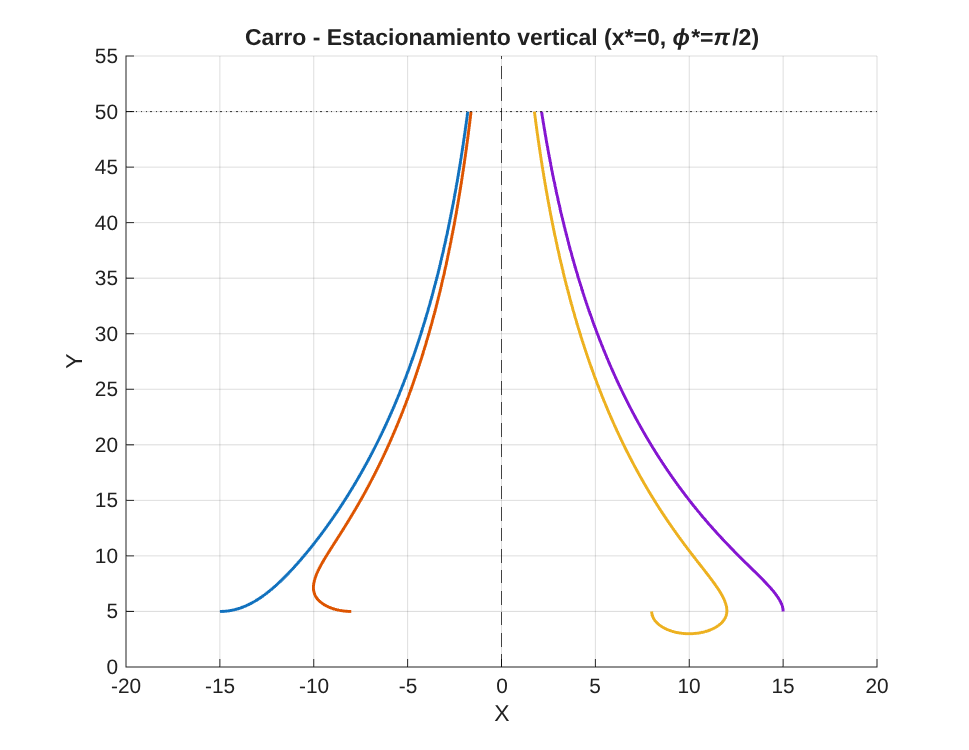
\includegraphics[width=\linewidth]{figs/car_parking.png}
  \caption{Estacionamiento vertical.}\label{fig:carpark}
\end{minipage}\hfill
\begin{minipage}{0.33\linewidth}\centering
  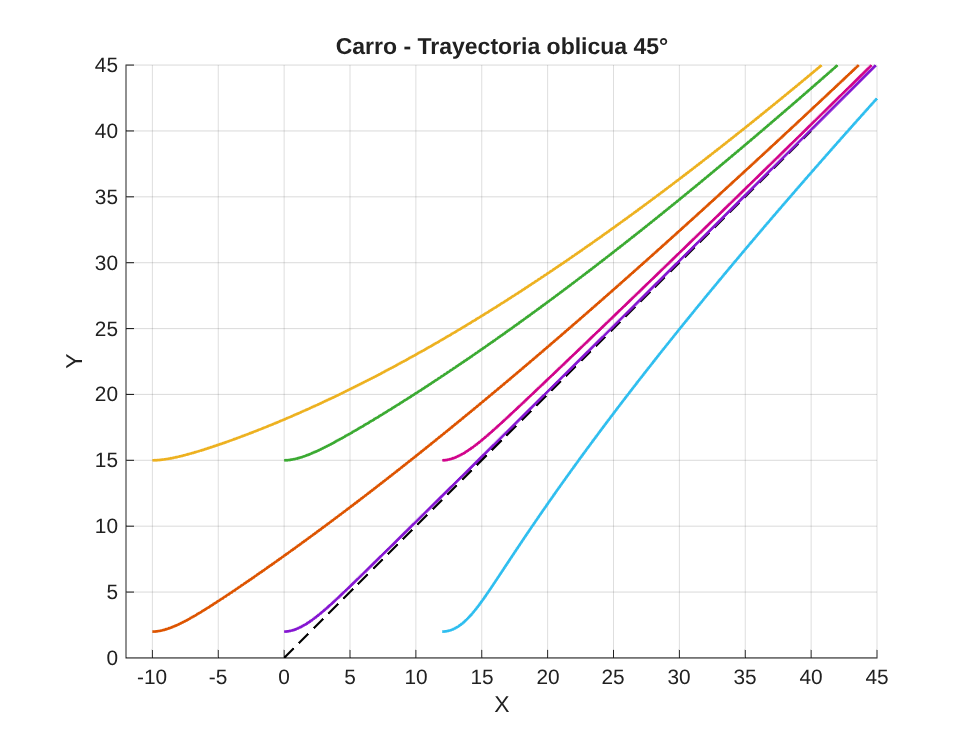
\includegraphics[width=\linewidth]{figs/car_oblique45.png}
  \caption{Oblicua $45^\circ$.}\label{fig:car45}
\end{minipage}\hfill
\begin{minipage}{0.33\linewidth}\centering
  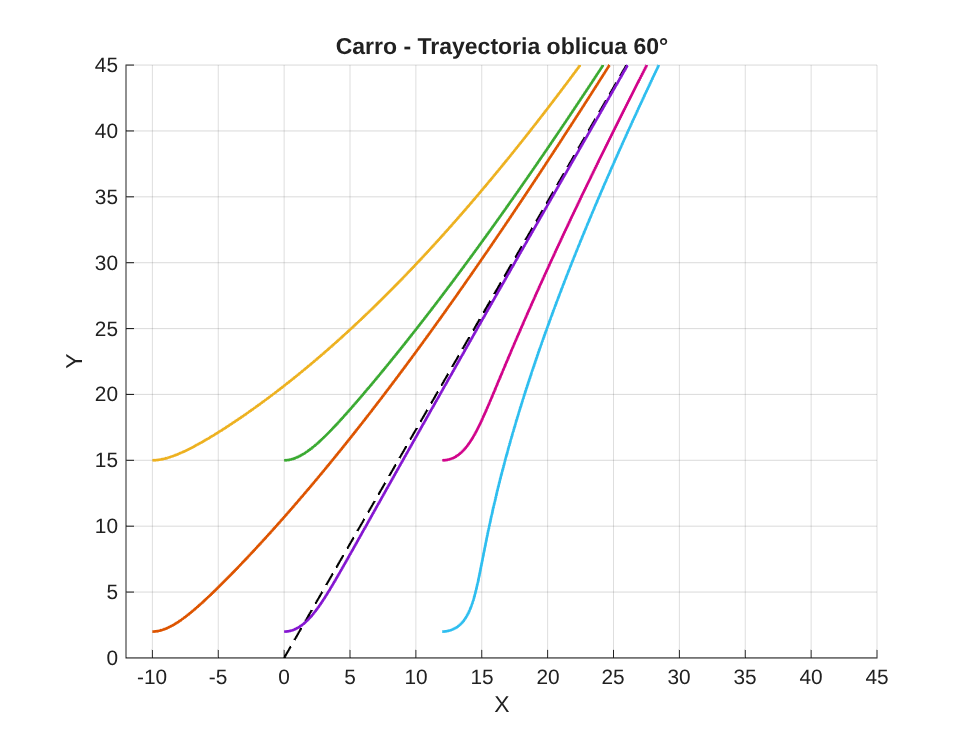
\includegraphics[width=\linewidth]{figs/car_oblique60.png}
  \caption{Oblicua $60^\circ$.}\label{fig:car60}
\end{minipage}
\end{figure}

\paragraph{Trayectoria circular.} Tratando la circular como el seguimiento de la
\emph{recta tangente local} más la \emph{acción anticipativa} de curvatura
$\delta^*=\operatorname{atan}(L/R)$, el carro recorre el círculo de radio $R=20$: se
mantiene sobre él partiendo del propio círculo y lo \emph{captura} partiendo desde fuera
(Fig.~\ref{fig:carcirc}).

\begin{figure}[H]
\centering
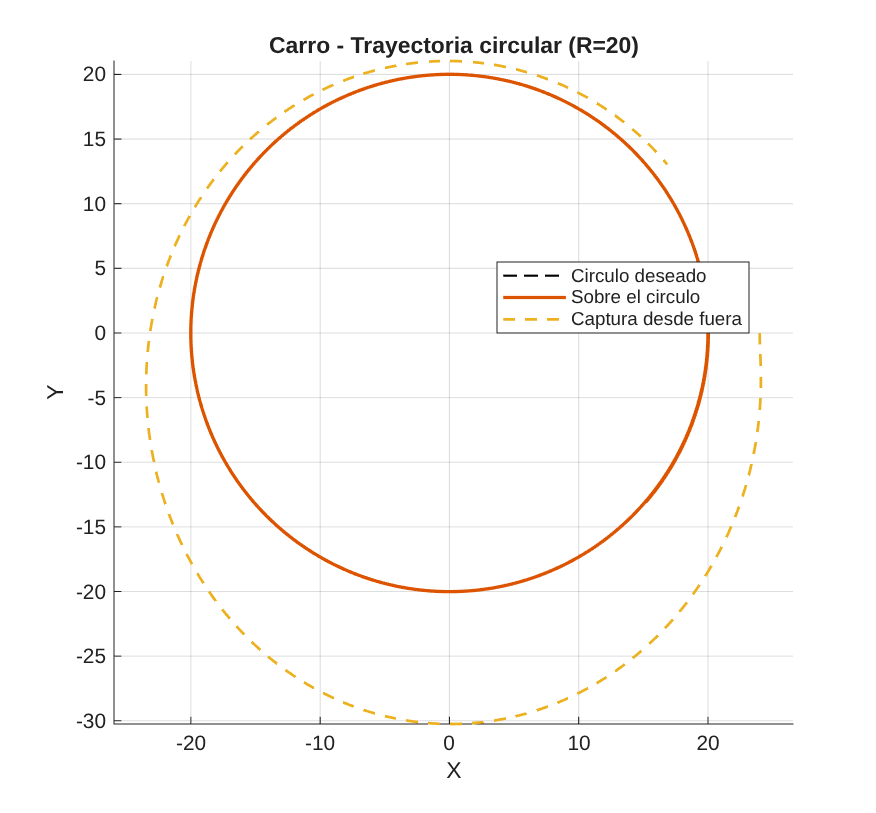
\includegraphics[width=0.52\linewidth]{figs/car_circular.png}
\caption{Seguimiento de trayectoria circular ($R=20$, sentido horario).}\label{fig:carcirc}
\end{figure}

\subsection{Robot tipo trailer}
\label{sec:trailer}
Con el modelo articulado de cuatro estados y la red entrenada por imitación de la ley
estabilizadora (MSE de ajuste $\approx 8\times10^{-3}$, Fig.~\ref{fig:trtrain}), el
trailer resuelve las tres trayectorias.

\paragraph{Estacionamiento vertical.} Partiendo de distintas posiciones y orientaciones
del remolque, el trailer maniobra hasta $x=0$ y queda \textbf{vertical}
($\theta_2\!\to\!\pi/2$), sin \emph{plegado del remolque} (Fig.~\ref{fig:trpark}); el neurocontrolador
gestiona el ángulo de articulación para reorientar el remolque.

\paragraph{Oblicua y circular.} Con las mismas referencias que el carro (pie de la
perpendicular y $\theta_2^*=\theta$ para la recta; tangente local más \emph{acción anticipativa}
de curvatura para el círculo), el trailer sigue la recta a $45^\circ$
(Fig.~\ref{fig:tr45}) y describe la trayectoria circular (Fig.~\ref{fig:trcirc}). En el
círculo, la trayectoria del remolque queda a un radio algo mayor que el deseado, porque
la curvatura efectiva del conjunto tractor--remolque depende de $L_1$ y $L_2$ (el
\emph{acción anticipativa} usa una aproximación con $L_1$).

\begin{figure}[H]
\centering
\begin{minipage}{0.48\linewidth}\centering
  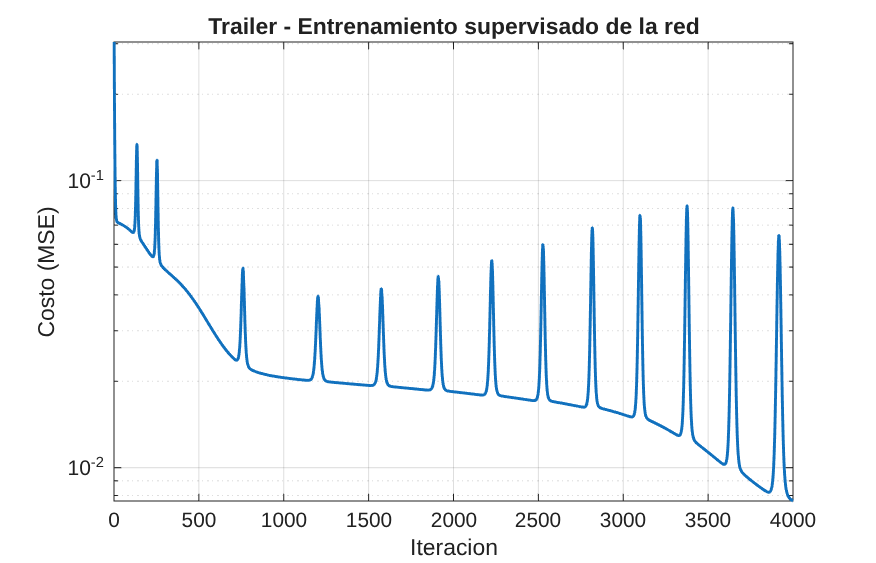
\includegraphics[width=\linewidth]{figs/trailer_training.png}
  \caption{Entrenamiento supervisado de la red del trailer.}\label{fig:trtrain}
\end{minipage}\hfill
\begin{minipage}{0.48\linewidth}\centering
  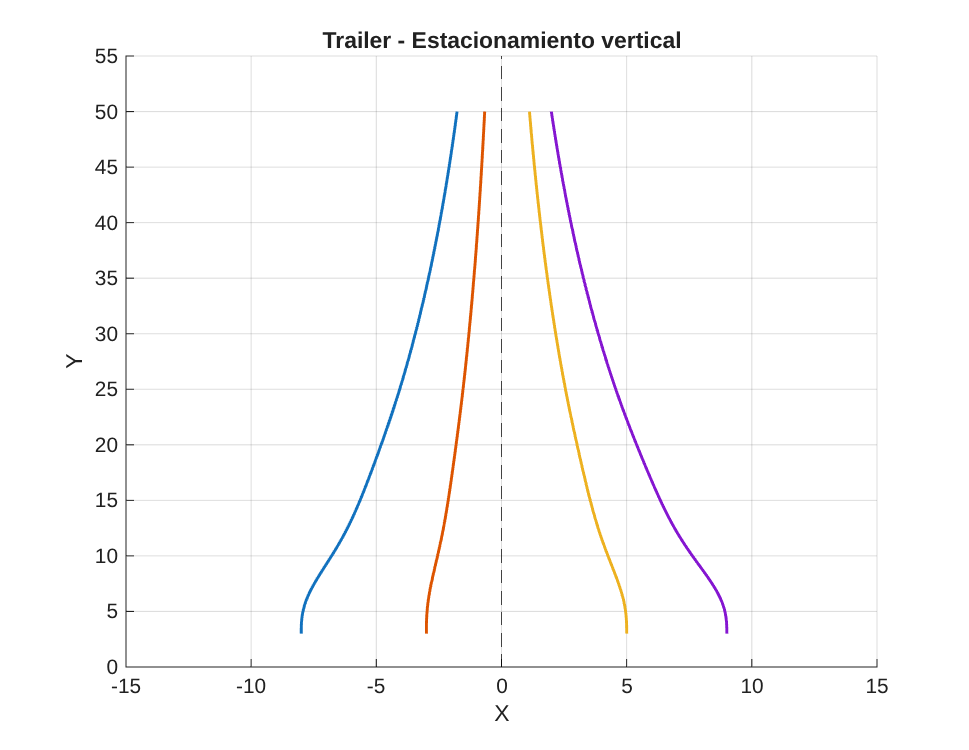
\includegraphics[width=\linewidth]{figs/trailer_parking.png}
  \caption{Estacionamiento vertical del trailer.}\label{fig:trpark}
\end{minipage}
\end{figure}

\begin{figure}[H]
\centering
\begin{minipage}{0.48\linewidth}\centering
  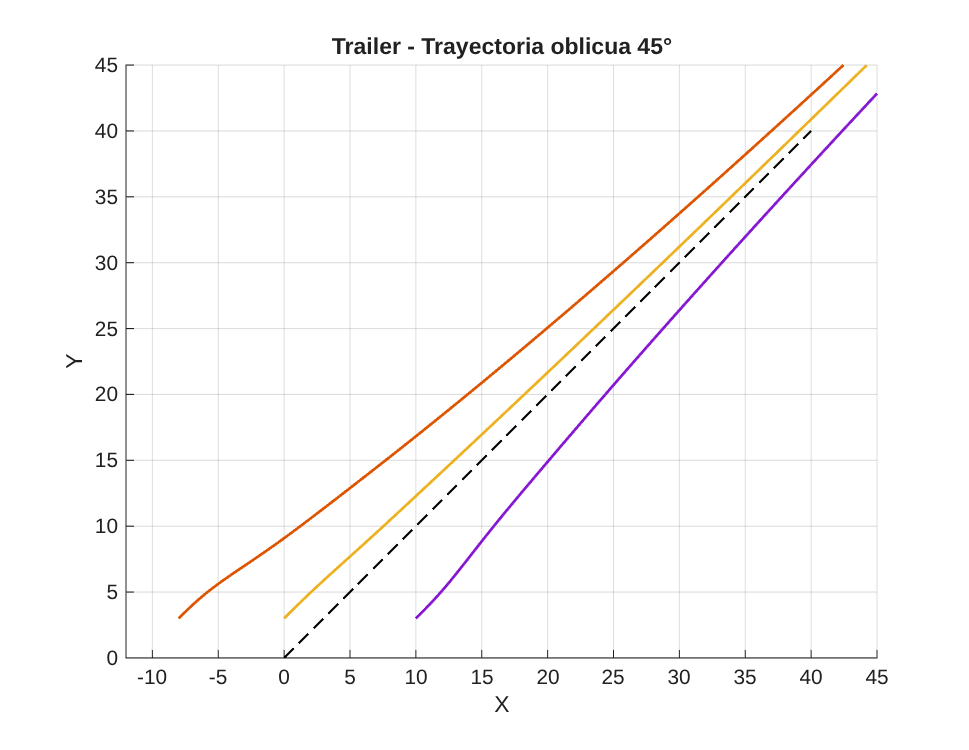
\includegraphics[width=\linewidth]{figs/trailer_oblique45.png}
  \caption{Trailer: oblicua $45^\circ$.}\label{fig:tr45}
\end{minipage}\hfill
\begin{minipage}{0.48\linewidth}\centering
  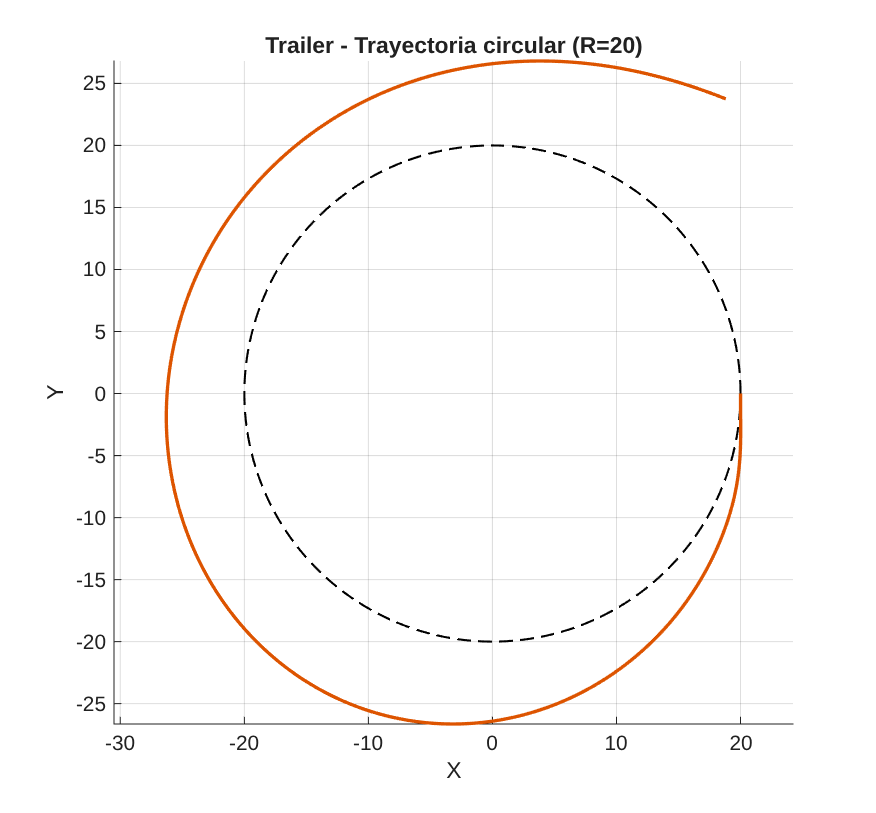
\includegraphics[width=\linewidth]{figs/trailer_circular.png}
  \caption{Trailer: trayectoria circular.}\label{fig:trcirc}
\end{minipage}
\end{figure}

% ================= CONCLUSIONES =================
\section{Conclusiones}
\begin{enumerate}
  \item \textbf{Una sola red basta para las tres trayectorias.} El neurocontrolador del
  carro, entrenado por BPTT solo para \emph{regulación} ($x^*=0,\ \phi^*=\pi/2$) pero
  cubriendo todas las orientaciones, resuelve el estacionamiento vertical, el seguimiento
  de rectas oblicuas ($45^\circ$ y $60^\circ$) y la trayectoria circular. Lo único que
  cambia entre trayectorias es \emph{cómo se define} la referencia $(x^*,\phi^*)$ en cada
  instante a partir de la geometría deseada.

  \item \textbf{La independencia de $y$ es la clave.} Como la señal de dirección $\delta$
  no depende de la coordenada $y$, el problema de seguimiento se reduce a regular el error
  de $x$ y de orientación; para las rectas se usa el pie de la perpendicular y para el
  círculo su recta tangente local más una \emph{acción anticipativa} de curvatura
  $\delta^*=\operatorname{atan}(L/R)$.

  \item \textbf{El entrenamiento BPTT requiere cuidados.} Por el horizonte largo, fueron
  necesarios el \emph{entrenamiento por etapas} incremental, la \emph{normalización} de entradas, el
  \emph{BPTT truncado} y el \emph{recorte de gradiente}; con ellos el costo converge de
  forma estable.

  \item \textbf{El trailer es un problema más difícil.} Al ser un sistema
  \emph{subactuado} (para reorientar el remolque hay que generar primero un ángulo de
  articulación con el tractor), el BPTT desde cero no convergió a una política
  satisfactoria. Se implementaron su modelo articulado de cuatro estados y el entrenador
  BPTT, se verificó que el modelo es controlable con una ley estabilizadora, y la red del
  trailer se obtuvo por \emph{aprendizaje supervisado} de esa ley: con ella el trailer
  estaciona en vertical y sigue las trayectorias oblicua y circular. Un entrenamiento
  BPTT plenamente convergente para el trailer queda como trabajo futuro (entrenamiento por etapas más
  largo, ventana de truncamiento y regularización).
\end{enumerate}

\appendix
\section{Archivos del proyecto}
Los experimentos se ejecutan con \code{Informe/exp/}: \code{car\_experiments.m} (tres
trayectorias del carro con la red \code{redcarro11}), \code{train\_car\_demo.m}
(convergencia del entrenamiento), \code{train\_trailer.m} + \code{trailer\_probe.m}
(entrenamiento BPTT del trailer) y \code{trailer\_experiments.m} (sus trayectorias). Las
figuras se guardan en \code{Informe/figs/}.

\end{document}
